\chapter{Opis rozwiązania}\label{chap:system_description}
\section{Redukcja problemu}\label{sec:reduction}
Jak już wspomniano w rozdziale \ref{chap:teoria}, uczenie głębokich sieci neuronowych w celu klasyfikacji obrazów dla dużych danych wejściowych jest zadaniem czasochłonnym.
Jednym ze sposobów redukcji tego czasu jest stosowanie archtektury konwolucyjnej (opisanej w \ref{sec:cnn}), która znacznie redukuje liczbę wag do nauczenia, a przy tym i czas obliczeń.
Nauczenie pojedynczej sieci konwolucyjnej wymaga wielu epok uczenia, najczęściej wykorzystując zrównoleleglenie obliczeń na kartach graficznych, np. wykorzystując bibliotekę CUDA w połączeniu z biblioteką TensorFlow.
Osiągnięcie skuteczności klasyfikacji na poziome 86\% dla zbioru CIFAR-10 dla przykładowej sieci zajmuje ok. $t_{cnn} = 3$ godzin dla typowej karty graficznej \textit{Nvidia Geforce GTX850M}. \cite{tensorflow2015-whitepaper}

W przypadku algorytmu genetycznego, jedna konwolucyjna sieć neruonowa jest jednym osobnikiem charakteryzowanym przez jego fenotyp, opisany w \ref{sec:fenotyp}.
Aby algorytm genetyczny skutecznie przeszukiwał przestrzeń poszukiwań, potrzebna jest stosunkowo duży rozmiar populacji $N$.
Jeśli wyznaczenie funkcji przystosowania byłoby jednoznaczne z wyznaczeniem skuteczności sieci po pełnym uczeniu, całkowity czas dla jednej iteracji dla $N = 100$:
 \begin{itemize}
	\item Przy sekwencyjnym uczeniu każdego osobnika wyniósłby $T_s = Nt_{cnn} = 300$ h$ =  12.5 $ dnia.
	\item Przy równoległym uczeniu każdego osobnika na $m = 10$ węzłach obliczeniowych wyniesie $T_p = \frac{T_s}{m} = 30$ h $= 1.25$ dnia.
\end{itemize}
Narzucając (oprócz kryterium stopu) maksymalną liczbę iteracji równą $I = 100$, w pesymistycznym przypadku dla obliczeń równoległych przy $m = 10$ całkowity czas obliczeń wyniósłby $T_c=IT_p=125$ dni.
W związku z ograniczonym czasem na przeprowadzenie badań oraz minimalizację kosztów obliczeń, czas ten musiał zostać znacznie zredukowany.

Jako rozwiązanie tego problemu zaproponowano:
\begin{enumerate}
	\item uczenie małych sieci, o ustalonych ramach i zmienności struktury wyznaczanej przez zmienną liczbę filtrów w warstwach konwolucyjnych (takich jak opisane w \ref{sec:fenotyp}).
	\item przyjęcie jako celu optymalizacji skuteczność sieci już po jednej epoce uczenia sieci.
\end{enumerate}

Dzięki przyjęciu takiego podejścia czas wyznaczania wartości funkcji przystosowania pojedynczego osobnika redukuje się do średniej wartości (wyznaczonej eksperymentalnie) około $t_{cnn} \approx 2.5 $ minut, co dla $m = 20$ sprowadza czas maksymalny działania algorytmu do $T_c \approx 21 h$.
Na tej zasadzie skonstruowano ekspetryment opisany w \ref{sec:actual_experiment}.

Po uczeniu sieci przez tak krótki czas, można sprawdzić czy wynik osiągany przez sieć już po jednej epoce uczenia ma związek z wynikiem uzyskanym po uczeniu dłuższym, np. dziesięciu epokach.
Proponowanym sposobem sprawdzenia powyżej sformułowanej hipotezy jest wzięcie najlepszego, środkowego i najgorszego osobnika z każdej iteracji algorytmu genetycznego i uczenie ich dłużej, np. przez 10 epok.
Ilość zmian kolejności najlepszy-środkowy-najgorszy dla przypadków 1- i 10- epokowego uczenia w stosunku do całkowiej liczby iteracji definuje stopień niepewności hipotezy, że istnieje wspominany związek.

Wybór 3 osobników ze 100 w każdej iteracji zmniejsza liczba wyznaczeń wartości nowej funkcji przystosowania z $N*I = 10000$ do $3*I = 300$, czyli ponad 33-krotnie, co pozwoliłoby uczyć przez 33 epoki w tym samym czasie.
W celu dalszej redukcji czasu i kosztów obliczeń zdecydowano się na nowe obliczenia dla 10-epok.

Należy pamiętać, że w tym eksperymencie nie szukamy nowych rozwiązań, a sprawdzamy inną funkcję przystosowania dla wybranego ich podzbioru.

\section{Sieć neuronowa jako osobnik algorytmu genetycznego}\label{sec:fenotyp}

Przykładową sięć neuronową powstającą w wyniku działania algorytmu przedstawiono na rys. \ref{fig:fenotyp}.
Na rysunku widać dwie następujące po sobie warstwy konwolucyjne, każda ze zmienną liczbą filtrów, dobieraną przez algorytm gentyczny.
Następująca po niej warstwa agregująca zmniejsza wymiar danych wejściowych dla kolejnych dwóch wartstw konwolucyjnych, dla których liczba filtrów również jest dobierana przez algorytm.
Po niej następuje warstwa w pełni połączonych 128 neuronów, za którą znajduje się warstwa 10 neurnów, każdy odpowiadający jednej klasie obrazka ze zbioru CIFAR-10.

Dzięki takiej architekturze osobnik może zostać sprametryzowany jako lista czterech liczb całowitych, nazywana dalej fenotypem, które można zakodować na 5 bitach każdą, przechodząc w ten sposób do genotypu.
Binarne kodowanie konieczne jest do wybranego sposobu krzyżowania osobników, opisanego w \ref{sec:genetic_ops}.
Zaproponowana sieć jest arbitralnie dobraną siecią, dla której bloki przedstawione na czerwono są ustalone, a ilośc filtrów w blokach przedstawionych na zielono jest zmienna.

\begin{figure}[h!tb]
	 \centering
	 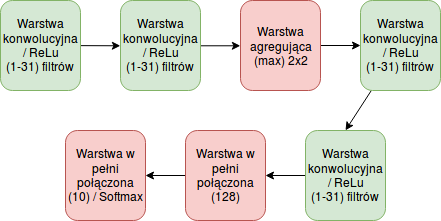
\includegraphics[width = 1.0\linewidth]{img/fenotyp}
	 \caption{Przedstawienie pojedynczego osobnika \\
              Źródło: praca własna}
	 \label{fig:fenotyp}
\end{figure}

Odgórne osiagi zbioru sieci ograniczone są przez elementy ustalone, tj. czerwone elementy na rys. \ref{fig:fenotyp}, stałą liczbę warstw konwolucyjnych (4) oraz granice w jakich zmieniają się liczby filtrów w tychże (1-31).
Zadaniem algorytmu genetycznego będzie maksymalizacja jakości klasyfikacji obrazów tak opisanych sieci po jednej epoce uczenia.
Przy tak dobranych parametrach osobnika możliwe jest wystąpienie zjawiska nadmiernego dopasowania do zbioru uczącego przez otrzymane sieci, w związku z brakiem zastosowania środków zapobiegawczych (takich jak dropout).

Funkcja przystosowania dla pojedynczego osobnika, jak już wspomniano w \ref{sec:reduction}, została określona jako skuteczność sieci po jednej epoce uczenia.
Nic nie stałoby jednak na przeszkodzie, aby dodać inne kryteria do funkcji przystosowania, np. gdyby zależało nam na uzyskaniu sieci która zajmuje mało pamięci moglibyśmy odjąć od funkcji przysotoswania odjąć odpowiednią karę proporcjonalną do sumy ilości wszystkich filtrów w wartswach.

\section{Operacje genetyczne algorytmu genetycznego}\label{sec:genetic_ops}
Spośród wymienionych w \ref{sec:ag} operacji genetycznych należało wybrać, jakie zaimplementować w programie realizującym algorytm genetczyny.
\subsection{Selekcja}
Wybranym w tej pracy sposobem selekcji jest sposób proporcjonalny, zwany również ruletkowym.
Każdy z osobników przypisany zostaje do obszaru ruletki, którego rozmiar jest proporcjonalny do wartości funkcji przystosowania tego osobnika.
Następnie $N$-krotnie kręci się ruletką, a pole, na które wypadnie, determiunje który z osobników przechodzi do puli potomków.
W ten sposób lepiej przystosowane osobniki mają większą szansę przejścia dalej i przekazania swoich genów.
W przypadku długotrwałego obliczania funkcji przystowania dodatkową zaletą takiego podejścia jest większa szansa na pojawienie się takich samych osobników (które nie zostaną poddane krzyżowaniu ani mutacji) w kolejnej iteracji algorytmu.
Z punktu widzenia efektywniejszego przeszukiwania przestrzeni dostępnych rozwiązań nie jest to zaletą, jednakże pozwala oszczędzić obliczeń dla już obliczonych punktów.

Tutaj metoda proporcjonalna została zaimplementowana w następujący sposób:

Powtórz $N$-krotnie:
\begin{enumerate}
  \item Sumowane są wartości funkcji przystowania $S(\mathbf{x})=\sum_{i=1}^{N}f(x_i)$ dla każdego $x_i$ w populacji
  \item Losowana jest losowa liczba z przedziału $r = (0,S(\mathbf{x}))$
  \item Znajdowane jest najmniejsze $i$, dla którego w danej sekwencji osobników $\sum_{i=1}^{N}x_i > r $
\end{enumerate}

\subsection{Krzyżowanie}
Przy implementacji algorytmu genetycznego wybrano krzyżowanie jednorodne.
Dla pary chromosomów rodzicielskich, które są w isotcie dwoma ciągami binarnymi o jednakowej długości, losowana jest binarna maska o tej samej długości.
Następnie następuje zamiana miejscami bitów oznaczonymi jako 1 w wylosowanej masce, w wyniku czego powstają dwa nowe chromosomy - potomkowie.
Działanie to w sposób schematyczny predstawiono na rys. \ref{fig:crossing}.
Rozważając poniższy przykład jako dwie warstwy konwolucyjne zakodowane na 4-bitach każdy, z rodziców $[12,3]$ oraz $[7,1]$ otrzymujemy z daną maską dwie nowe sieci z warstwami: $[5,3]$ oraz $[14,1]$.

\begin{figure}[h!tb]
	 \centering
	 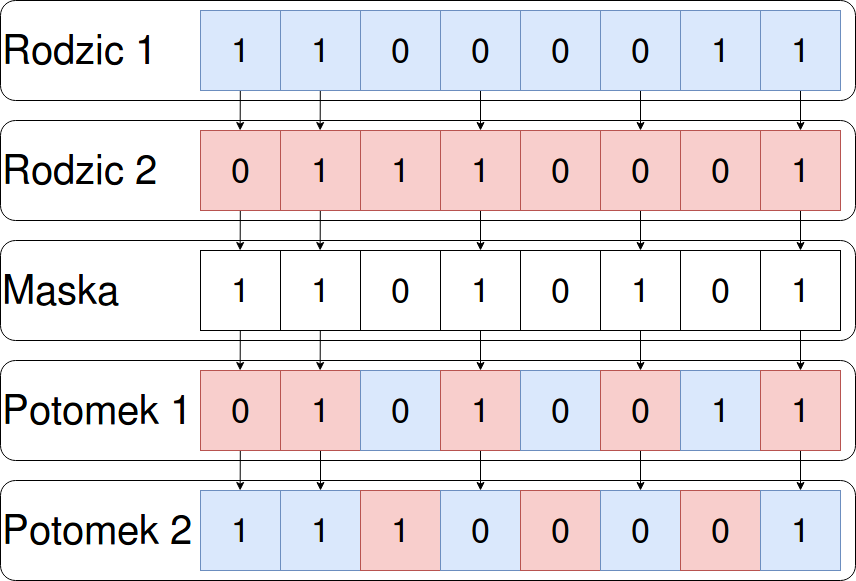
\includegraphics[width = 1.0\linewidth]{img/crossing}
	 \caption{Krzyżowanie jednorodne \\
              Źródło: praca własna}
	 \label{fig:crossing}
\end{figure}

\subsection{Mutacja}
Sposób mutacji wykorzystany w tej pracy tożsamy jest ze zmianą wartościowo-równomierną.
Dokonywana jest ona na fenotypie osobnika.
Jeżeli mutacja danego osobnika zachodzi, to:
\begin{itemize}
  \item Losowo wybierana jest liczba ze zbioru $\lbrace 0, 1, 2, 3 \rbrace$, która determinuje, który parametr będzie zmeiniany
  \item Następuje wylosowanie nowej wartości dla wybranego parametru z dopuszczalengo zbioru liczb całkowitych $\lbrace 1..31 \rbrace$, który zastępuje starą wartość
\end{itemize}

\subsection{''Naprawianie'' osobników}\label{sec:individual_fix}
Istnieje pewne prawdopodobieństwo, że w wyniku krzyżowania otrzymamy osobnika, dla którego jeden lub więcej parametrów przyjmie wartość zero.
Rozwiązać ten problem można na dwa sposoby:
\begin{enumerate}
  \item Na poziomie algorytmu genetycznego - zamieniając otrzymane 0 losową lub najbliższą (1) dopuszczalną wartością\label{bullet:genetic_fix}
  \item Na poziomie konstruowania sieci neuronowej - jeżeli warstwa zawiera 0 filtrów to jest pomijana w sekwencyjnym budowaniu modelu sieci.
\end{enumerate}
W pracy zdecydowano się zastosować się podejście \ref{bullet:genetic_fix} z zastępowaniem 0 przez 1, ze względu na prostotę implementacyjną.

\subsection{Substytucja}
Zastosowana w algorytmie technika substucji osobników rodzicielskich przez potomków jest strategią z reprodukcją częściową.
W celu zmiejszenia ilości obliczeń potomkowie nie są oceniani do momentu, kiedy staną się rodzicami w następnym pokoleniu.
Z tego powodu zastosowano połączenie strategii elitarnej (pozostanwienie najlepszych osobników z poprzedniej iteracji) z zastępowaniem losowo wybranych osobników (losowo wybierane są nowe osobniki z puli potomków).
Pozwala to dodatkowo zaoszczędzić obliczeń dla przeniesionej z poprzedniej iteracji elity przy jednoczesnym zachowaniu różnorodności genetycznej pochodzącej od losowo wybranych potmków.
Dodatkowo, w stosunku do pełnej reprodukcji (z wymianą całej populacji), algorytm szybciej znajduje lepsze rozwiązania.

\section{Architektura eksperymentu}
W toku przygotowywania eksperymentów powstał system napisany w języku Python\cite{CS-R9526}.
Najważniejsze jego elementy zostały wyróżnione na rys. \ref{fig:system_overview}

\begin{figure}[h!tb]
	 \centering
	 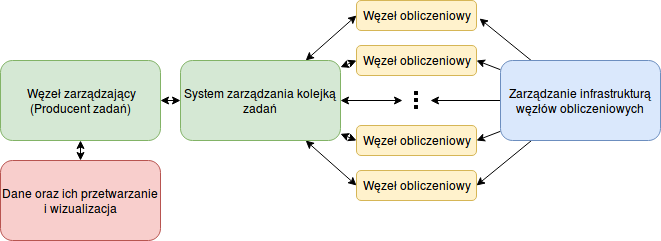
\includegraphics[width = 1.0\linewidth]{img/system_overview}
	 \caption{Całokształt systemu przeprowadzania eksperymentu \\
              Źródło: praca własna}
	 \label{fig:system_overview}
\end{figure}

Każdy z powyżej przedstawionych elementów zostanie omówiony dalej.
Poniżej, na rys. \ref{fig:folder_structure} przedstawiono strukturę katalogów projektu:

\begin{figure}[h!tb]
	 \centering
	 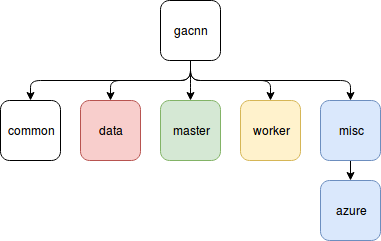
\includegraphics[width = 0.7\linewidth]{img/folder_structure}
	 \caption{Struktura katalgoów projektu systemu eksperymentu\\
              Źródło: praca własna}
	 \label{fig:folder_structure}
\end{figure}

Całość projektu zorganizowano w katalogi tak, aby zgrupować pliki źródłowe powiązane z konkretnymi blokami funkcjonalmi z rys. \ref{fig:system_overview}.
Bloki oznaczone na obydwu rysunkach tym samym kolorem są swoimi odpowiednikami.
W związku z tym:
\begin{itemize}
  \item katalog \textit{gacnn} jest korzeniem, również nazwą repozytorium kodu źródłowego.
        Jego nazwa jest abrewiacją angielskich odpowiedników nazw algorytm genetyczny i konwolucyjna sień neuronowa.
  \item katalog \textit{common} zawiera elementy potrzebne możliwie przez każdy z innych modułów
  \item katalag \textit{data} przechowuje zebrane przez węzeł zarządzający dane oraz skrypty służące do ich przetwarzania i wizualizacji
  \item katalog \textit{master} zawiera wszystkie programy, które mogą być węzłem zarządajacym, oraz system zarządzania kolejką zadań
  \item katalog \textit{worker} zawiera oprogramowanie uruchamiane na każdym z węzłów obliczeniowych
  \item katalog \textit{misc} zawiera pomocnicze skrypty służące do tworzenia i przygotowywania węzłów obliczeniowych
  \item katalog \textit{azure} zawiera skrypty j.w. przeznaczone konkretnie do tworzenia instancji węzłów obliczeniowych na platformie Microsoft Azure
\end{itemize}

\subsection{Elementy wspólne}
Wspólne elementy autorskiego kodu używane zarówno przez węzeł zarządający, jak i przez węzły obliczeniowe, to definicje dwóch klas:
\begin{itemize}
  \item Klasa \textit{Job} - opisuje zadane przekazywane przez węzeł zarządzający do systemu kolejkowego i dalej do węzła obliczeniowego.
        W istocie swej jest to struktura przechwoująca 3 elementy:
        \begin{itemize}
          \item osobnika (reprezentowanego przez obiekt klasy \textit{Individual}), dla którego należy wyznaczyć funkcję przystosowania
          \item liczbę epok uczenia sieci neuronowej
          \item ziarno dla generatora pseudolosowego
        \end{itemize}
  \item Klasa \textit{Individual} - opisuje pojedynczego osobnika, tj. pojedynczą strukturę sieci neuronowej.
        Przechwouje ona 4 informacje:
        \begin{itemize}
          \item Fenotyp osobnika - lista 4 liczb opisujących liczbę filtrów w odpowiednich warstwach sieci
          \item Przystosowanie osobnika - wartość funkcji przystosowania osobnika.
                Dla algorytmu optymalizującego strukturę konwolucyjnej sieci neuronowej jest to skuteczność klasyfikacji zbioru testowego przez nauczoną sieć.
          \item Ostateczna uzyskana wartość funkcji kosztu (\textit{loss function}) po uczeniu - w celu informacyjnym
          \item Historię uczenia sieci - przechowuje wartości przystosowania i funkcji kosztu po każdej epoce uczenia sieci, przechowywane w celach informacyjno-diagnostycznych
        \end{itemize}
\end{itemize}


\subsection{Węzeł zarządzający}

Węzłem zarządzającym nazywany będzie program, który korzysta z opisanego w \ref{sec:queue_system} systemu kolejkowego do rodzielania swoich zadań i odbierania wyników.
Jego głównym zadaniem jest typowanie osobników, dla których ma zostać wyliczona funkcja przystosowania.
Dla potrzeb wspomnianych w \ref{sec:reduction} funkcji przystosowania dla uczenia 1- i 10- epokowego konieczne było stworzenie dwóch programów zarządających:
\begin{enumerate}
  \item Węzeł typujący osobniki do wyliczenia na podstawie działania algorytmu genetycznego dla uczenia 1-epokowego - plik \textit{gentic\_algorithm.py}\label{list:genetic}
  \item Węzeł typujący najlepsze, środkowe i najgorsze osobniki z każdej iteracji algorytmu genetycznego dla uczenia 10-epokowego - plik \textit{full\_learning.py}\label{list:full}
\end{enumerate}
Obydwa z wyżej wymienionych węzłów korzystają z pomocniczych funkcji do zapisywania odebranych od węzłów obliczeniowych danych - plik \textit{csv\_handling.py}.

Węzeł opisany powyżej w punkcie \ref{list:genetic} został napisany tak, by możliwie łatwo można było regulować parametry algorytmu.
Poniżej przedstawiono ich listę:
\begin{itemize}
  \item liczba osobników $N$
  \item wymiarowość przestrzeni poszukiwań - liczba warstw konwolucyjnych $n$
  \item zakres przestrzeni poszukiwań - liczba bitów przypadających na kodowanie jednej warstwy $m$
  \item prawdopodobieństwo krzyżowania - $p_{c}$
  \item prawdopodobieństwo mutacji - $p_{m}$
  \item maksymalna liczba iteracji
  \item maksymalna liczba iteracji bez poprawy
  \item liczba najlepszych osobników przechodzących do kolejnego pokolenia - $ N_{k} = 30$
  \item minimalna poprawa $\epsilon$
  \item ziarno genetora pseudolosowego - domyślnie 1337
\end{itemize}

Po ustawieniu wyżej wymienionych parametrów, program działa następująco:

\begin{enumerate}
  \item Ustawia zadane ziarno generatora losowego. Przyczny, dla których to robi, opisano w \ref{sec:replicativity}.
  \item Jeśli nie istnieje, tworzy plik .csv do przechowywania danych, gdzie każdy wpis zawiera:
  \begin{itemize}
    \item Numer iteracji
    \item Genotyp osobnika w formie zakodowanej
    \item Wartość funkcji przystosowania
    \item Wartość funkcji kosztu
  \end{itemize}
  \item Jeżeli istnieje plik .csv z danymi z niedokończonego działania programu, wczytuje je.
  \item Jeżeli nie wczytano żadnych danych, następuje inicjalizacja populacji. Losowo generowanych jest $N$ osobników.
  \item Dopóki nie osiagnięto kryterium stopu (maksymalna liczba iteracji bez poprawy wyniku lub maksymalna liczba iteracji osiągnięte)
  \begin{enumerate}
    \item Przygotowuje listę zadań dla systemu kolejkowego - dla każdego osobnika tworzy jedno zadanie, które w jednym zdaniu brzmi: ''Ucz tego osobnika przez 1 epokę z takim ziarnem generatora pseudolosowego''.
    \item Oblicza wartość funkcji przystosowania dla całej populacji korzystając z metody \textit{evaluate(jobs)} systemu kolejkowania zadań.
    \item Sortuje osobniki według wartości funkcji przystowania
    \item Zapisuje dane z tej iteracji do pliku csv
    \item Sprawdza najlepszy wynik i czy w tej iteracji nastąpiła poprawa - jeśli nie, zwiększa licznik iteracji bez poprawy
    \item Za starą popuację podstawia nową uzyskaną w wyniku:
    \begin{enumerate}
      \item selekcji
      \item krzyżowania
      \item mutacji
      \item ''naprawiania'' osobników
      \item substytucji
    \end{enumerate}
    Wszystkie z powyższych odbywają się jak opisano w \ref{sec:genetic_ops}
  \end{enumerate}
\end{enumerate}

W wyniku działania powyższego skryptu otrzymujemy plik csv zawierający wszystkie osobniki z wszystkich iteracji działania algorytmu genetycznego.
Dane te są przetwarazne dalej w celu wizualizacji, jak również przez skrypt \textit{full\_learning.py}, który również jest węzłem zarządającym, a działa następująco:
\begin{enumerate}
  \item Wczytuje osobniki zapisane w pliku .csv przez algorytm genetycznych
  \item Z każdej iteracji wybiera najlepszego, środkowego i najgorszego osobnika
  \item Dla każdego wybranego osobnika tworzy zadanie, które w jednym zdaniu brzmi: ''Ucz tego osobnika przez 1 epokę z takim ziarnem generatora pseudolosowego''.
  \item Oddelegowuje zadania do systemu kolejkowania zadań.
  \item Zbiera wyniki i zapisuje je do innego pliku.
\end{enumerate}
Ten skrypt wyznacza inną funkcję przystosowania dla tych samych osobników - skuteczność po 10 epokach uczenia, w porównaniu do 1-epokowego uczenia.

\subsection{System kolejkowania zadań}\label{sec:queue_system}
W celu maksymalnego przyspieszenia obliczeń, dokonano zrównoleglenia obliczania funkcji przystosowania dla każdego osobnika.
Ze względu na ograniczoną liczbę jednostek obliczeniowych mogących jednocześnie przetwarzać żądania, zaprojektowano system kolejkowy.
Schemat tego systemu przedstawiono na rys. \ref{fig:queue_system}
\begin{figure}[h!tb]
	 \centering
	 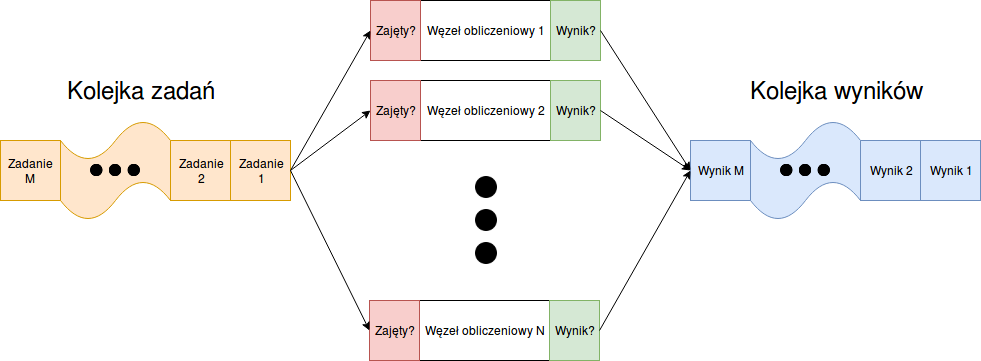
\includegraphics[width = 1.1\linewidth]{img/kolejkowanie}
	 \caption{System kolejkowania obliczeń \\
              Źródło: praca własna}
	 \label{fig:queue_system}
\end{figure}

Implementacja systemu kolejkowego zawarta jest w pliku \textit{queue\_handling.py}.
Zawiera on następujące elementy:

\begin{itemize}
  \item Interfejs \textit{Worker} będącą reprezentacją pojedynczego węzła obliczeniowego.
  \item Klasę \textit{RemoteWorker} dziedziczącą po klasie \textit{Worker}, służącą do delegowania zadań do zdalnej maszyny wirtulnej wykonującej obliczenia.
  \item Klasę \textit{LevyWorker} dziecziczącą po klasie \textit{Worker}, lokalnie wyznaczającą wartość funkcji Levego, używana przy testowaniu działania algorytmu genetycznego jak opisano w \ref{sec:levy_test}.
  \item Klasę \textit{WorkManager} będącą właściwą implementacją systemu kolejkowania.
\end{itemize}

Interfejs \textit{Worker} zawiera następujące metody:
\begin{itemize}
  \item \textit{is\_available()} - mówi, czy dany węzeł może przyjmować teraz zadania
  \item \textit{assign\_job(job)} - przypisuje do danego węzła przekazane jako argument zadanie do oblicznia
  \item \textit{has\_result()} - odpytuje węzeł, czy posiada już wynik obliczeń
  \item \textit{get\_result{}} - zwraca odebrany od węzła wynik obliczeń
  \item \textit{free\_worker()} - zwalnia węzeł oznaczając go jako gotowy do rozpoczęcia dalszych obliczeń
  \item \textit{get\_current\_job()} - zwraca aktualnie zlecone węzłowi zadanie
\end{itemize}

Właściwą implementacją systemu kolejkowego jest klasa \textit{WorkManager}.
System kolejkowy przechowuje wewnętrznie listę dostepnych węzłów obliczeniowych.
Jedyną publiczną metodą tej klasy jest funkcja \textit{evaluate(jobs)}, która jako argument przyjmuje listę zadań do wykonania.
Dla przypadku obsługi węzłów zdalnych system kolejkowy:

\begin{enumerate}
  \item Wyszukuje dupilkaty wśród otrzymanych zadań i zawęża listę zadań do unikalnego zbioru\label{list:duplicates}
  \item Dopóki liczba uzyskanych wyników jest mniejsza od liczby zleconych zadań:
    \begin{enumerate}
      \item Sprawdza plik \textit{workers} z listą adresów IP potencjalnych węzłów
      \item Próbuje połączyć się z węzłami zgodnie z procedurą opisaną w \ref{sec:communication}.
      \item Dodaje każdy zgłaszający się węzeł do listy węzłów i oznacza go jako wolny.
      \item Rodziela zadadania każdemu z węzłów, dla każdego węzła z listy:
        \begin{enumerate}
          \item Sprawdza czy ten węzeł jest oznaczony jako wolny i czy są dostępne zadania.
                Jeśli nie, przechodzi do kolejnego węzła i powtarza obecny krok.
          \item Pobiera zadanie z puli dostępnych zadań
          \item Próbuje przypisać pobrane zadanie do tego węzła (może się to nie udać np. z powodu utraty połączenia sieciowego).
          \item Jeśli powyższy krok się nie powiódł, przywraca zadanie do puli zadań, a niedziałący węzeł jest usuwany z listy węzłów.
        \end{enumerate}
      \item Odpytuje każdy zajęty węzeł o wyniki w następujący sposób:\label{enum:second_worker_check}
      \begin{enumerate}
        \item Odpytuje węzeł czy wynik jest dostępny.
              Jeśli nie, przechodzi do kolejnego węzła i powtarza obecny krok.
        \item Pobiera od węzła jego wynik i zadanie. Zapisuje je do słownika, gdzie zadanie jest kluczem, a wynik wartością.
        \item Oznacza węzeł jako wolny.
        \item Jeśli któryś z powyższych kroków się nie powiódł, przywraca zadanie węzła do puli i usuwa go z listy węzłów.
      \end{enumerate}
      \item W celu zmniejszenia obciążenia sieci przy komunikacji z węzłami, odczekuje sekundę przed kolejną iteracją.
    \end{enumerate}
  \item Przywraca usunięte w punkecie \ref{list:duplicates} duplikaty, przepisując odpowiednie wyniki z policzonych zadań ze słownika zadanie-wynik.
\end{enumerate}

W przypadku testu dla lokalnie oblicznaje wartości funkcji Levego opisanego w \ref{sec:levy_test} system ten, z pewnymi modyfikacjami, również może zostać wykorzystany.
Oblczenia wykonywane są lokalnie i dostępne są natychmiast po zleceniu zadania, w związku z czym:
\begin{itemize}
  \item lista węzłów zawiera tylko jeden węzeł \textit{LevyWorker} i nie jest w żaden sposób modyfikowana
  \item pominięte zostaje opóźnienie odciążające sieć
\end{itemize}

\subsection{Protokół komunikacji ze zdalnymi węzłami}\label{sec:communication}

Komunikacja ze zdalnymi węzłami odbywa się przez protkół TCP/IP z wykorzystaniem interfejsu \textit{socket} języka Python.

Schemat wymiany komunikatów przedstawiony został na rysunku \ref{fig:komunikacja}
\begin{figure}[h!tb]
	 \centering
	 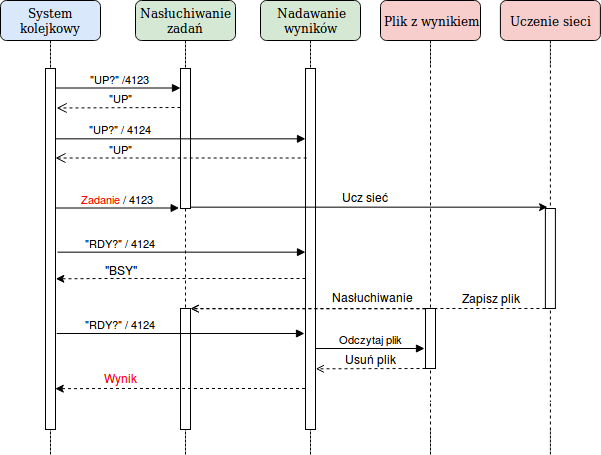
\includegraphics[width = 1.0\linewidth]{img/komunikacja}
	 \caption{Schemat wymiany komunikatów pomiędzy systemem kolejkowym a węzłami obliczeniowymi \\
              Źródło: praca własna}
	 \label{fig:komunikacja}
\end{figure}

Widoczne u góry bloki komunikują się ze sobą zgodnie ze shematem.
Pierwszy (niebieski) blok reprezentuje komunikujący się z węzłem obliczeniowym system kolejkowania zadań.
Pozostałe 4 bloki stanowią podystem pojedynczego węzła obliczeniowego.
Na zielono zaznaczono obiekty komunikujące się przez sieć, natomiast na czerwono zaznaczono bloki niedostępne bezpośrednio z poziomu węzła zarządzającego.

Sama komunikacja przebiega w następujący sposób.
\begin{enumerate}
  \item System kolejkowy sprawdza, czy pod zadanym adresem IP rzeczywiście znajduje się węzeł obliczeniowy.
  Sprawdzenie to polega na przesłaniu tekstowo zapytania ''UP?'' na obydwa otwarte porty węzła obliczeniowego.
  Jeżeli w odpowiedzi z obydwu portu dostaje komunikat ''UP'', dodaje węzeł do swojej wewnętrznej listy węzłów i nie powtarza więcej tej komunikacji do momentu, kiedy znowu będzie potrzeba dodania tego węzła do listy.
  \item Jeżeli poprzedni punkt przebiegł pomyślnie, węzeł jest gotowy do przyjęcia zadania.
  System kolejkowy przesyła spakowany przy pomocą modułu \textit{Pickle} obiekt klasy \textit{Job} na port 4123, który jest używany do akceptacji zadań.\label{list:job}
  \item Następnie cyklicznie (co sekundę, jest to wspominane w \ref{sec:queue_system} opóźnienie przesyłane jest zapytanie na port 4124 czy jest już wynik poprzez komunikat ''RDY?''.
  Jeżeli wynik jeszcze nie jest dostępny, odsyłana jest odpowiedź ''BSY'' oznaczająca dalsze trwanie obliczeń.\label{list:result}
  W przeciwnym wypadku przesyłany jest spakowany przy pomocą modułu \textit{Pickle} obiekt klasy \textit{Individual} zawierający w sobie wyniki obliczeń.
  \item System kolejkowy następnie powtarza kroki \ref{list:job} i \ref{list:result} tak długo, jak posiada zadania do rodzielenia, lub dopóki nie nastąpi nieoczekiwany błąd.
\end{enumerate}

\subsection{Węzeł obliczeniowy}\label{sec:worker_node}

Przez węzeł obliczeniowy rozumieć będziemy komputer lub maszynę wirtualną z dostępem do sieci komputerowej, w której znajduje się węzeł zarządzający.
Dodatkowym wymaganiem na taki węzeł jest możliwość uruchomienia na nim skryptów \textit{listener\_results.py} oraz \textit{listener\_jobs.py}, przy czym ten drugi powinen być cyklicznie uruchamiany w przypadku wystąpienia błędu.
Implikuje to obecność na danej maszynie interpretera języka Python w wersji 3 wraz z odpowiednimi bibliotekami, tj. \textit{TensorFlow}\cite{tensorflow2015-whitepaper}, \textit{Keras}\cite{chollet2015keras} oraz \textit{Numpy}\cite{ascher.dubois.hinsen.hugunin.oliphant-1999-np}.
Co więcej, urządzenie to musi mieć możlwość przyjmowania połączeń od systemu kolejkowego na portach TCP 4123 oraz TCP 4124.

Zadaniem węzła obliczeniowego jest przyjęcie zadania od systemu kolejkowego, wykonanie go i dostarczenie wyniku, również na żądanie systemu kolejkowego, przy spełnianiu wyspecyfikowanego w \ref{sec:communication} protokołu komunikacyjnego.
W związku z tym kod uruchamiany na węźle został rodzielony na 3 pliki źródłowe, każdy odpowiedzialny za jedno z tych zadań.

Pierwszym z nich jest \textit{listener\_jobs.py}.
Działa on według nastepującego schematu:
\begin{enumerate}
  \item Ustawia socket nasłuchujący połączeń na porcie TCP/4123
  \item W nieskończonej pętli:
  \begin{enumerate}
    \item Akceptuje przychodzące połączenie i odbiera dane
    \item Jeżeli w przychodzących danych występuje komunikat ''UP?'' odsyła komunikat ''UP'', zamyka połączenie i pomija resztę kroków w tym przebiegu pętli.
    \item Zamyka połączenie od systemu kolejkowego.
    \item Rozpakowuje przychodzące dane i sprawdza czy otrzymano obiekt klasy \textit{Job}, w przeciwnym wypadku generuje wyjątek i zakańcza działanie programu.
    \item Przekazuje sterowanie do funkcji \textit{eval\_network(...)} z parametrami odczytanymi z otrzymanego obiektu.
  \end{enumerate}
\end{enumerate}

Na czas uczenia sieci proces nie nasłuchuje połączeń - przyjęto założenie projektowe, że to system zarządzający koleką przechwouje informację, że ten węzeł własnie pracuje i zostanie zwolniony po odebraniu wyników.

Kolejny plik, tj. \textit{evan\_cnn.py}, zawiera jedną metodę, która oblicza funkcję przystosowania osobnika, poprzez skonsturowanie modelu sieci, uczenie go zbiorem uczącym oraz walidację na zbiorze testowym obrazków ze zbioru CIFAR-10.
Bardziej szczegołowo:
\begin{enumerate}
  \item Ustawia zadane ziarno generatora losowego. Przyczny, dla których to robi, opisano w \ref{sec:replicativity}.
  \item Ładuje do pamięci zbiór danych CIFAR-10. Jeżeli skrypt jest uruchamiany pierwszy raz, pobiera ów zbiór z internetu.
  \item Buduje model sieci neuronowej taki jak przedstawiono na rys. \ref{fig:fenotyp}.
        Budowanie modelu jest uniwersalne dla różnych długości fenotypu, tj. różnej zadanej ilości warstw konwolucyjnych.
        Warstwa agregująca zostanie wstawiona w połowie , czyli dla 4 warstw za 2. warstwą.
  \item Uczy uzyskany model korzystając z optymalizatora \textit{RMSProp} przez zadaną liczbę epok. Otrzymaną historię uczenia przechwouje w odpowiednim polu obiektu klasy \textit{Individual}.\label{list:training}
  \item Sprawdza skuteczność uzyskanej nauczonej sieci na zbiorze testowym, j.w. zapisując uzyskaną skuteczność i wartosć funkcji kosztu w odpowiednich polach.\label{list:check}
  \item Pakuje uzupełniony przez powyższe operacje obiekt klasy \textit{Individual} przy pomocy modułu \textit{pickle} i zapisuje wynik w pliku ''result''.
\end{enumerate}

Przy przeprowadzaniu eksperymentów zaobserwowano niedeterministyczne występowanie wyjątku \textit{MemoryError} oznaczającego zużycie całej dostępnej pamięci i brak miejsca na zaalokowanie nowej, powodujący zakończenie działania programu.
Prawdopodobą przyczyną jest błąd programistyczny w jednej z użytych bibliotek.
Zastosowanym sposobem obejścia tego problemu jest ponowne uruchomienie skryptu przez inny skrypt.

Trzeci plik \textit{listener\_results.py} odpowiedzialny jest za przesyłanie wyników na żądanie systemu kolejkowego lub informowanie, że nie są one jeszcze dostępne.
Program ten realizuje następujące kroki:
\begin{enumerate}
  \item Ustawia socket nasłuchujący połączeń na porcie TCP/4124
  \item W nieskończonej pętli:
  \begin{enumerate}
    \item Akceptuje przychodzące połączenie i odbiera dane
    \item Jeżeli w przychodzących danych występuje komunikat ''UP?'' odsyła komunikat ''UP''. Jeżeli warunek nie jest spełniony, sprawdzany jest warunek poniżej.
    \item Jeżeli w przychodzących danych występuje komunikat ''RDY?'' sprawdza czy jest dostępny plik z wynikami. Jeżeli nie, przesyła w opdowiedzi komunikat ''BSY''. Jeżeli jest, wysyła odczytany plik z wynikami.
    \item Zamyka połączenie z systemem kolejkowym.
  \end{enumerate}
\end{enumerate}

Do poprawnego działania węzła obliczeniowego konieczne jest współbieżne uruchomienie skryptów \textit{listener\_results.py} oraz \textit{listener\_jobs.py}.
Co więcej, w związku ze wspomnianymi niedeterministycznymi błędami przy obliczniu wartości funkcji przystowania, program zbierający zadania powinien być restartowany po każdym krytycznym błędzie.
W związku z wykorzystaniem maszyn wirtualnych opartych o system Linux, w celu spełnienia dwóch powyższych warunków napisany został skrypt w języku Bash o nazwie \textit{starter.sh}.
Aby węzeł obliczeniowy zaczął działać, należy uruchomić w tle ten skrypt.
Jego działanie opisać można następująco:
\begin{enumerate}
  \item Usuń plik z wynikami - zakładamy, że startujemy od nowa i nie powinno być wyników - realizowane przez komendę \textit{rm result}
  \item Wyłącz działające procesy nasłuchujące zadań i wyników - realizowane przez komendę \textit{pkill python}
  \item Uruchom w tle i uniezależnij od procesu rodzica skrypt \textit{listener\_results.py}
  \item W nieskończonej pętli:
  \begin{enumerate}
    \item Uruchom skrypt \textit{listener\_jobs.py} i czekaj na jego wykonanie
    \item Poczekaj 10 sekund - oczekiwanie przed kolejnym uruchomieniem programu w przypadku, gdyby zajęty port TCP/4123 nie został jeszcze zwolniony.
  \end{enumerate}
\end{enumerate}

Tak złożony system spełnia warunki postawione na węzeł obliczeniowy.
Schematyczną jego reprezentację przedstawiono na rys. \ref{fig:worker_node}.
Każdy element wewnątrz prostokąta reprezentuje jeden z plików w folderze \textit{worker}.
Linia przerwyana pomiędzy blokami \textit{listener\_results.py} a \textit{starter.sh} oznacza jedno uruchomienie.
Z kolei cykl pomiędzy \textit{listener\_jobs.py} a \textit{starter.sh} symbolizuje ponowne uruchamianie skryptu.
Na niebiesko zaznaczano współbieżnie dziające skrypty komunikujące się z siecią.
Na czerwono zaznaczono elementy wykorzystywane wewnętrznie przez węzeł obliczeniowy.
Na zielono zaznaczono element rozpoczynający działanie systemu.
\begin{figure}[h!tb]
	 \centering
	 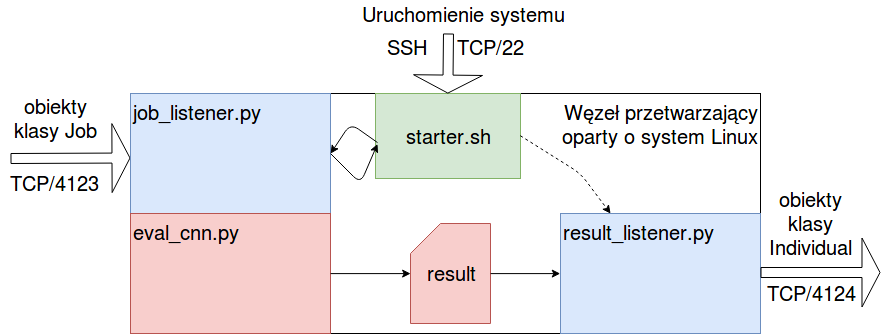
\includegraphics[width = 1.0\linewidth]{img/worker_node}
	 \caption{Schemat systemu obsługi zadań \\
              Źródło: praca własna}
	 \label{fig:worker_node}
\end{figure}

\subsection{Zarządanie infrastrukturą węzłów obliczeniowych}\label{sec:azure}
Opisanym w \ref{sec:worker_node} węzłem obliczeniowym może być, jak wspomniano tamże, dowolna maszyna z systemem operacyjnym wspierającym uruchamianie równolegle procesów interpretra języka Python.
Dobrym rozwiązaniem okazują się być maszyny wirtualne z systemem Linux w chmurze.
Poniżej przedstawiono listę kilku dostawców takiego rozwiązania, których rozważano przy do stworzenia infrasturktury węzłów obliczeniowych:

\begin{itemize}
  \item Amazon Web Services
  \item Microsoft Azure
  \item Google Cloud Platform
  \item DigtalOcean
  \item Oktawave
  \item OVH
\end{itemize}

Na dzień dzisiejszy firma \textit{Microsoft} oferuje 100\$ kredytu do wykorzystania dla studentów w celach badawczych, dlatego rozwiązanie to zostało wykorzystane do utworzenia 20 instancji maszyn wirtualnych, które wykorzystano jako węzły obliczeniowe.
Subskrypcja dla studentów ma jednak pewne ograniczenia.
W trakcie prototypowego tworzenia infrastruktury napotkano ogranieczenie możliwości działających vCPU w jednym regionie do 4.
Tym samym nie można było korzystać z maszyn wirtualnych wyposażonych w więcej vCPU, między innymi z przedstawionych w tabeli \ref{tab:gpu_optimized_vms}

\begin{table}[h!tb]
\centering
\small
\caption{Maszyny wirtualne zopytmalizowane pod kątem głębokiego uczenia. Żródło: \cite{gpuvms2018}}\label{tab:gpu_optimized_vms}
\begin{tabularx}{\linewidth}[c]{|l|X|X|X|X|X|X|X|X|X|} \hline
  Rozmiar & vCPU & Pamięć [GiB] & Pojemność tymczasowa (SSD) [GiB] & GPU & Maksymalnie dysków z danymi & Maksymalnie kart sieciowych \\ \hline
  Standard\_ND6s & 6 & 112 & 736 & 1 & 12 & 4 \\ \hline
  Standard\_ND12s &	12 & 224 & 1474 & 2 & 24 & 8 \\ \hline
  Standard\_ND24s & 24 & 448 & 2948 & 4 & 32 & 8 \\ \hline
 	\noalign{\smallskip}
\end{tabularx}
\vspace{-8pt}
\end{table}

Blok zarządzania infrastukturą węzłów obliczeniowych widoczny na rys. \ref{fig:system_overview} po prawej stronie może reprezentować człowieka - operatora, który ręcznie utworzy wszystkie instancje korzystając z dostępnego na stronie \url{http://portal.azure.com} interfejsu WWW.
Na rys. \ref{fig:azure} przedstawiono interfejs webowy \textit{Microsoft Azure}.

\begin{figure}[h!tb]
	 \centering
	 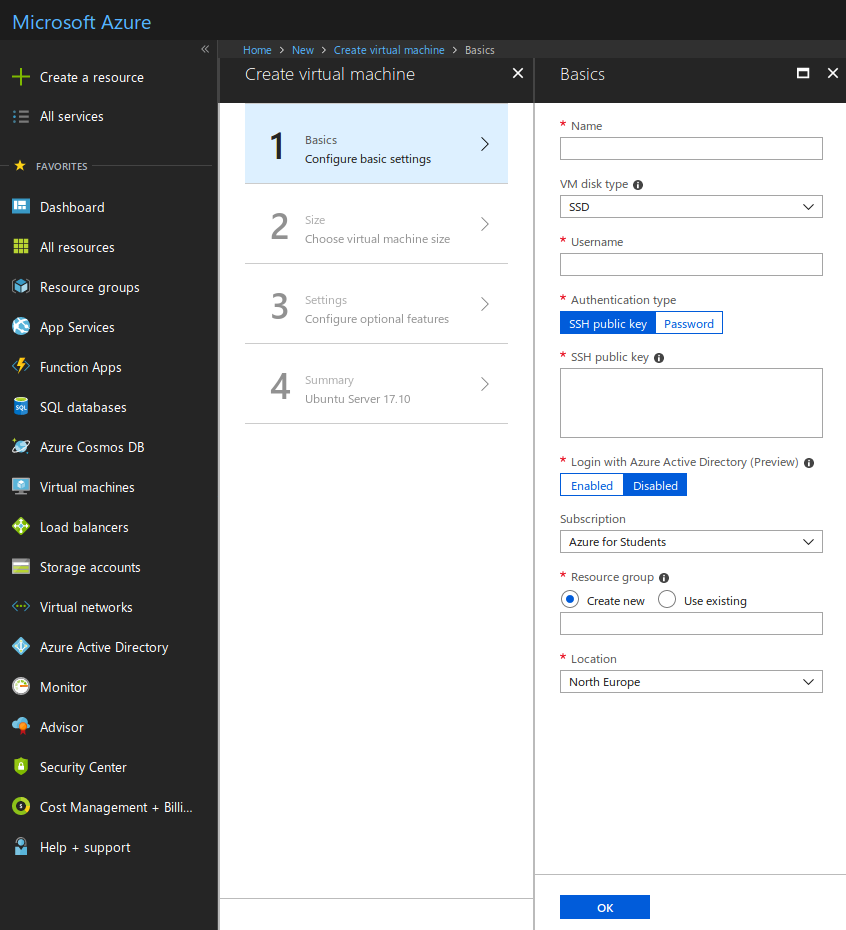
\includegraphics[width = 1.0\linewidth]{img/azure}
	 \caption{Interfejs Microsoft Azure - tworzenie maszyny wirtualnej \\
              Źródło: praca własna}
	 \label{fig:azure}
\end{figure}

Jak widać, oprócz początkowego wybrania obrazu (tutaj wybrano Ubuntu 17.10) należy przejść przez 4 etapy, gdzie musi podjąć następujące kroki:
\begin{enumerate}
  \item Wprowadzić nazwę maszyny wirtualnej, np. \textit{Worker1}
  \item Wprowadzić dane do logowania przez ssh: nazwę użytkownika i klucz publiczny
  \item Wybrać lub stworzyć grupę zasobów (nazwano grupę \textit{gacnn})
  \item Lokalizację - przy czym należy pamiętać o limicie 4 vCPU na lokalizację
  \item Wybrać rozmiar maszyny wirtualnej - tutaj wybrano rozmiar nazwany \textbf{DS1\_v2} o następujących parametrach:
  \begin{itemize}
    \item liczba vCPU: 1
    \item Pamięć RAM: 3.5 GB
    \item Rozmiar lokalnego SSD: 7 GB
    \item Cena: 41.41€ za miesiąc (0.0557€ za godzinę)
  \end{itemize}
  \item Raz w każdym regionie stworzyć zestaw reguł zapory ogniowej (\textit{Network Security Group}) i dodać do niego regułę akceptującą połączenia na portach TCP: 4123-4124
  \item Przypisać utworzony powyżej zestaw reguł do tworzonej maszyny wirtualnej
  \item Wyłączyć nieporzebną opcję diagnostyki uruchamiania (\textit{Boot Diagnostics})
  \item Zatwierdzić utworzenie maszyny wirtualnej
\end{enumerate}
Rozwiązanie takie jest jednak czasochłonne i niefektywne, przejście przez wszystkie etapy przy dużym poziomie koncentracji operatora zajmuje ok. ~3 minuty, co oznacza, że utworzenie 20 maszyn wirtualnych zajęłoby około godziny.

Rozwiązaniem tego problemu jest wykrzostanie narzędzia \textit{Azure CLI}, czyli interfejs linni komend dla Azure.
Pozwala on na zarządzanie maszynami wirtualnymi przy pomocy komend wydawanych z linii poleceń lub z poziomu skryptów napisanych w języku \textit{Bash} lub \textit{PowerShell}.
Zostały napisane dwa skrypty w języku bash.
Pierwszy to \textit{spawner.sh}, który tworzy 20 maszyn wirtualnych w 5 regionach po 4 maszyny za pomocą następującej komendy wywoływanej w pętli:\\

\begin{lstlisting}
az vm create --location $region --name $name
             --resource-group gacnn --size Standard_DS1_v2
             --image Canonical:UbuntuServer:17.10:latest
             --admin-username admin
             --ssh-key-value id_rsa.pub
             --no-wait
\end{lstlisting}

Zmienna \textit{region} przyjmuje jedną z wartości: \textit{northeurope, westeurope, francecentral, eastus, eastus2}.

Zmienna \textit{name} tworzona jest w następujący sposób:

\begin{lstlisting}
name=$region"worker"$i
\end{lstlisting}

Dzięki tej tworzone jest 20 maszyn o rozmiarze \textbf{DS1\_v2} o unikalnych nazwach.
Każda przypisywana jest do grupy zasobów \textit{gacnn}.
Wytwarzane są na podstawie najnowszego dostępnego obrazu \textit{Ubuntu Server 17}.
Logowanie do takiej maszyny możliwe jest z loginem admin i wyłącznie przy pomocy klucza publicznego z pliku \textit{id\_rsa.pub}.

Po utworzeniu maszyn należy im również otworzyć odpowiednie porty, odbywa się to przy pomocy komendy wywoływanej w pętli:
\begin{lstlisting}
az vm open-port --port 4123-4124 --resource-group gacnn --name $name
\end{lstlisting}

Z tak przygotowanymi maszynami można się połączyć przy pomocy programu, który pozowala obsługiwać wiele terminali naraz, np. \textit{Cluster SSH}.
Adresy IP maszyn odczytać można korzystając już z interfejsu WWW Azure, wyświetlając wszystkie dostępne maszyny wirtualne i ich publiczne adresy IP.
Poniższe kroki można w ten sposób wykonywać na 20 maszynach jednoecześnie.

Dalsze przygotowanie środowiska dla węzła obliczeniowego polega na:
\begin{enumerate}
  \item pobraniu programu \textit{python3-pip}
  \item instalacja za jego pomocą bibliotek \textit{numpy, tensorflow, keras}.
  \item sklonowanie repozytorium umieszczonego pod adresem \url{https://github.com/opiechow/gacnn}
  \item przejście do katlogu gacnn/worker
  \item uruchomienie skrytu starer.sh
\end{enumerate}

Po tych operacjach węzeły obliczeniowe działają i czekają na zadania od systemu kolejkowego.
Można zmodyfikować plik \textit{starter.sh}, aby przekierować wyjście ze skryptu \textit{listener\_jobs.py} na standarowe wyjście, co pozwoli obserwować proces uczenia w terminalu.
Przykładowy widok dla sześciu węzłów obliczeniowych przedstawiono na rys. \ref{fig:wip}

\begin{figure}[h!tb]
	 \centering
	 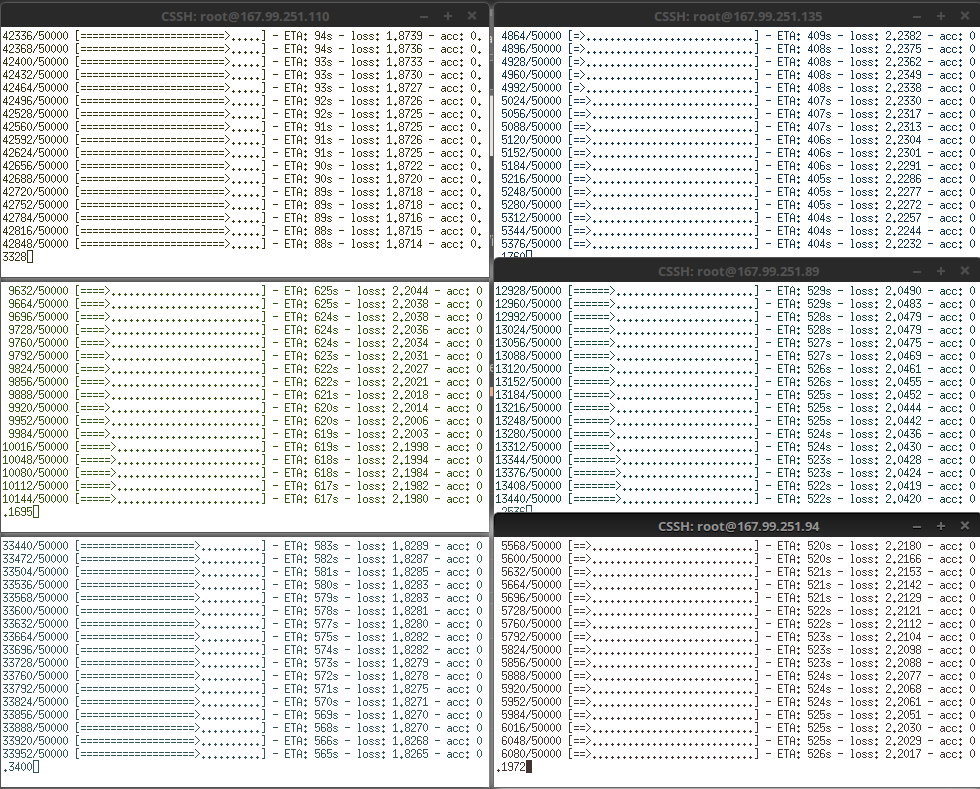
\includegraphics[width = 1.0\linewidth]{img/wip}
	 \caption{6 węzłów obliczeniowych w trakcie pracy \\
              Źródło: praca własna}
	 \label{fig:wip}
\end{figure}

\section{Replikatywność badań}\label{sec:replicativity}
Zarówno w przypadku działania algorytmu genetycznego, jak i w przypadku uczenia sieci neuronowych, występuje wiele operacji, które z założenia powinnny być niedeterministyczne.
Poniżej przedstawiono listę tych operacji dla algorytmu genetycznego:
\begin{itemize}
  \item Losowe generowanie początkowej populacji algorytmu genetycznego
  \item Selekcja ruletkowa
  \item Losowe dobieranie osobników w pary rodzicielskie
  \item Zachodzenie krzyżowania z pewnym prawdopoboieństwem
  \item Losowanie maski w krzyżowaniu równomiernym
  \item Zachodzenie mutacji z pewnym prawdopodobieństwem
  \item Losowanie parametru do zmutowaniu
  \item Losowanie nowej wartości mutowanego parametru
  \item Losowanie części populacji przechodzącej do kolejnej iteracji
\end{itemize}

W przypadku uczenia sieci neuronowych losowo inicjalizowane są początkowe wagi w sieci.

Aby zapewnić replikatywność badań, w toku pisania systemu dbano o zachowanie kontroli nad stanem początkowym generatora liczb pseudolosowych.
W tym celu zarówno przed uruchomieniem algorytmu genetycznego jak i uczeniem sieci ustawiane jest ziarno generatora losowego.
W przypadku węzła zarządającego ziarno jest jednym z parametrów ustawianym przed uruchomieniem algorytmu.
W przypadku węzłów obliczeniowych ziarno dla generatora odbierane jest razem z zadaniem do policzenia.

W przypadku algorytmu genetycznego używany jest generator z wbudowanego w język \textit{Python} modułu \textit{random}, ustawienie ziarna nie jest skomplikowane - wystarczy jedna linia kodu.
W przypadku uczenia sieci neuronowych wszzystkie operacje losowe ukryte są w działaniu funkcji biblioteki \textit{Keras}.
Procedura ustawiania ziarna dla wszystkich generatorów dostępna jest w dokumentacji biblioteki. \cite{chollet2015keras}

Poważną wadą dbania o replikatywność jest wymuszenie na \textit{TensorFlow} działania wyłącznie na jednym wątku, gdyż uniemożliwia to korzystanie z korzyści oferowanych przez uczenie sieci przy pomocy GPU i technologii CUDA.
Aby umożliwić działanie systemu w tymi technologiami, kryterium stopu uzależniono od wariancji wyników uzyskanych dla takiej samej sieci korzystając z różnych wartości ziarna generatora liczb losowych.

W przypadku przedstawionych poniżej eksperymentów nie korzystano z uczenia GPU, a z 20 maszyn wirtualnych z jednym vCPU każda.
Ziarno ustawiane było wg. opisanej powyżej procedury, zatem wszystkie badania powinny być reprodukowalne.
